\newcommand*{\skypesocialsymbol} {%
  \protect\raisebox{-0.085em}{%
\protect\begin{tikzpicture}[y=0.08em,x=0.08em,xscale=0.022,yscale=-0.022, inner sep=0pt, outer sep=0pt]
\protect\path[fill=color2,even odd rule] (487.6550,288.9690) .. controls (489.0610,278.5690) and
  (489.8700,267.9960) .. (489.8700,257.2330) .. controls (489.8700,128.0770) and
  (384.5990,23.3610) .. (254.7670,23.3610) .. controls (241.8630,23.3610) and
  (229.2120,24.4210) .. (216.9010,26.4410) .. controls (194.8280,12.0570) and
  (168.5590,3.6740) .. (140.2880,3.6740) .. controls (62.7660,3.6740) and
  (0.0000,66.4820) .. (0.0000,143.9800) .. controls (0.0000,172.1780) and
  (8.2990,198.3740) .. (22.5900,220.3690) .. controls (20.6650,232.3860) and
  (19.6810,244.6920) .. (19.6810,257.2290) .. controls (19.6810,386.4050) and
  (124.8980,491.1100) .. (254.7660,491.1100) .. controls (269.4230,491.1100) and
  (283.6930,489.6840) .. (297.5620,487.1780) .. controls (319.1120,500.5470) and
  (344.4960,508.3260) .. (371.7080,508.3260) .. controls (449.2100,508.3260) and
  (512.0010,445.5020) .. (512.0010,368.0120) .. controls (511.9980,338.7190) and
  (503.0410,311.4840) .. (487.6550,288.9690) -- cycle(276.7400,429.5960) ..
  controls (202.0340,433.4870) and (167.0750,416.9590) .. (135.0500,386.9050) ..
  controls (99.2850,353.3370) and (113.6520,315.0500) .. (142.7900,313.1040) ..
  controls (171.9120,311.1590) and (189.3980,346.1160) .. (204.9410,355.8400) ..
  controls (220.4650,365.5280) and (279.5340,387.6000) .. (310.7350,351.9320) ..
  controls (344.7100,313.1040) and (288.1410,293.0120) .. (246.6760,286.9300) ..
  controls (187.4730,278.1640) and (112.7260,246.1370) .. (118.5410,183.0230) ..
  controls (124.3580,119.9490) and (172.1230,87.6090) .. (222.3910,83.0470) ..
  controls (286.4680,77.2300) and (328.1820,92.7540) .. (361.1760,120.9070) ..
  controls (399.3270,153.4360) and (378.6840,189.8010) .. (354.3770,192.7270) ..
  controls (330.1660,195.6360) and (302.9730,139.2230) .. (249.5860,138.3750) ..
  controls (194.5590,137.5110) and (157.3690,195.6360) .. (225.3000,212.1590) ..
  controls (293.2660,228.6640) and (366.0500,235.4450) .. (392.2610,297.5760) ..
  controls (418.4900,359.7130) and (351.5070,425.7010) .. (276.7400,429.5960) --
  cycle;
\protect\end{tikzpicture}}%
  ~}

\documentclass[11pt,a4paper,roman]{moderncv}        % possible options include font size ('10pt', '11pt' and '12pt'), paper size ('a4paper', 'letterpaper', 'a5paper', 'legalpaper', 'executivepaper' and 'landscape') and font family ('sans' and 'roman')


% moderncv themes
\moderncvstyle{classic}                             % style options are 'casual' (default), 'classic', 'oldstyle' and 'banking'
\moderncvcolor{green}                               % color options 'blue' (default), 'orange', 'green', 'red', 'purple', 'grey' and 'black'
%\renewcommand{\familydefault}{\sfdefault}         % to set the default font; use '\sfdefault' for the default sans serif font, '\rmdefault' for the default roman one, or any tex font name
\nopagenumbers{}                                  % uncomment to suppress automatic page numbering for CVs longer than one page

% character encoding
\usepackage[utf8]{inputenc}                       % if you are not using xelatex ou lualatex, replace by the encoding you are using
%\usepackage{CJKutf8}                              % if you need to use CJK to typeset your resume in Chinese, Japanese or Korean

% adjust the page margins
\usepackage[scale=0.77]{geometry}
%\setlength{\hintscolumnwidth}{3cm}                % if you want to change the width of the column with the dates
%\setlength{\makecvtitlenamewidth}{10cm}           % for the 'classic' style, if you want to force the width allocated to your name and avoid line breaks. be careful though, the length is normally calculated to avoid any overlap with your personal info; use this at your own typographical risks...

% personal data
\name{Mario}{Lamberti}
\title{Curriculum Vit\ae}                               % optional, remove / comment the line if not wanted
%\address{+39 340 42 61 266}{mario.lamberti31@gmail.com}{Anno di nascita: 31 Gennaio 1993}% optional, remove / comment the line if not wanted; the "postcode city" and and "country" arguments can be omitted or provided empty
\phone[mobile]{+39~340~4161266}                   % optional, , remove / comment the line if not wanted
\email{mario.lamberti31@gmail.com}                               %  remove / comment the line if not wanted

\extrainfo{\skypesocialsymbol mario.lamberti31 \\
			Date of birth: 31 January 1993 \\ 
			Place of birth: Salerno (SA), Italy}


\begin{document}
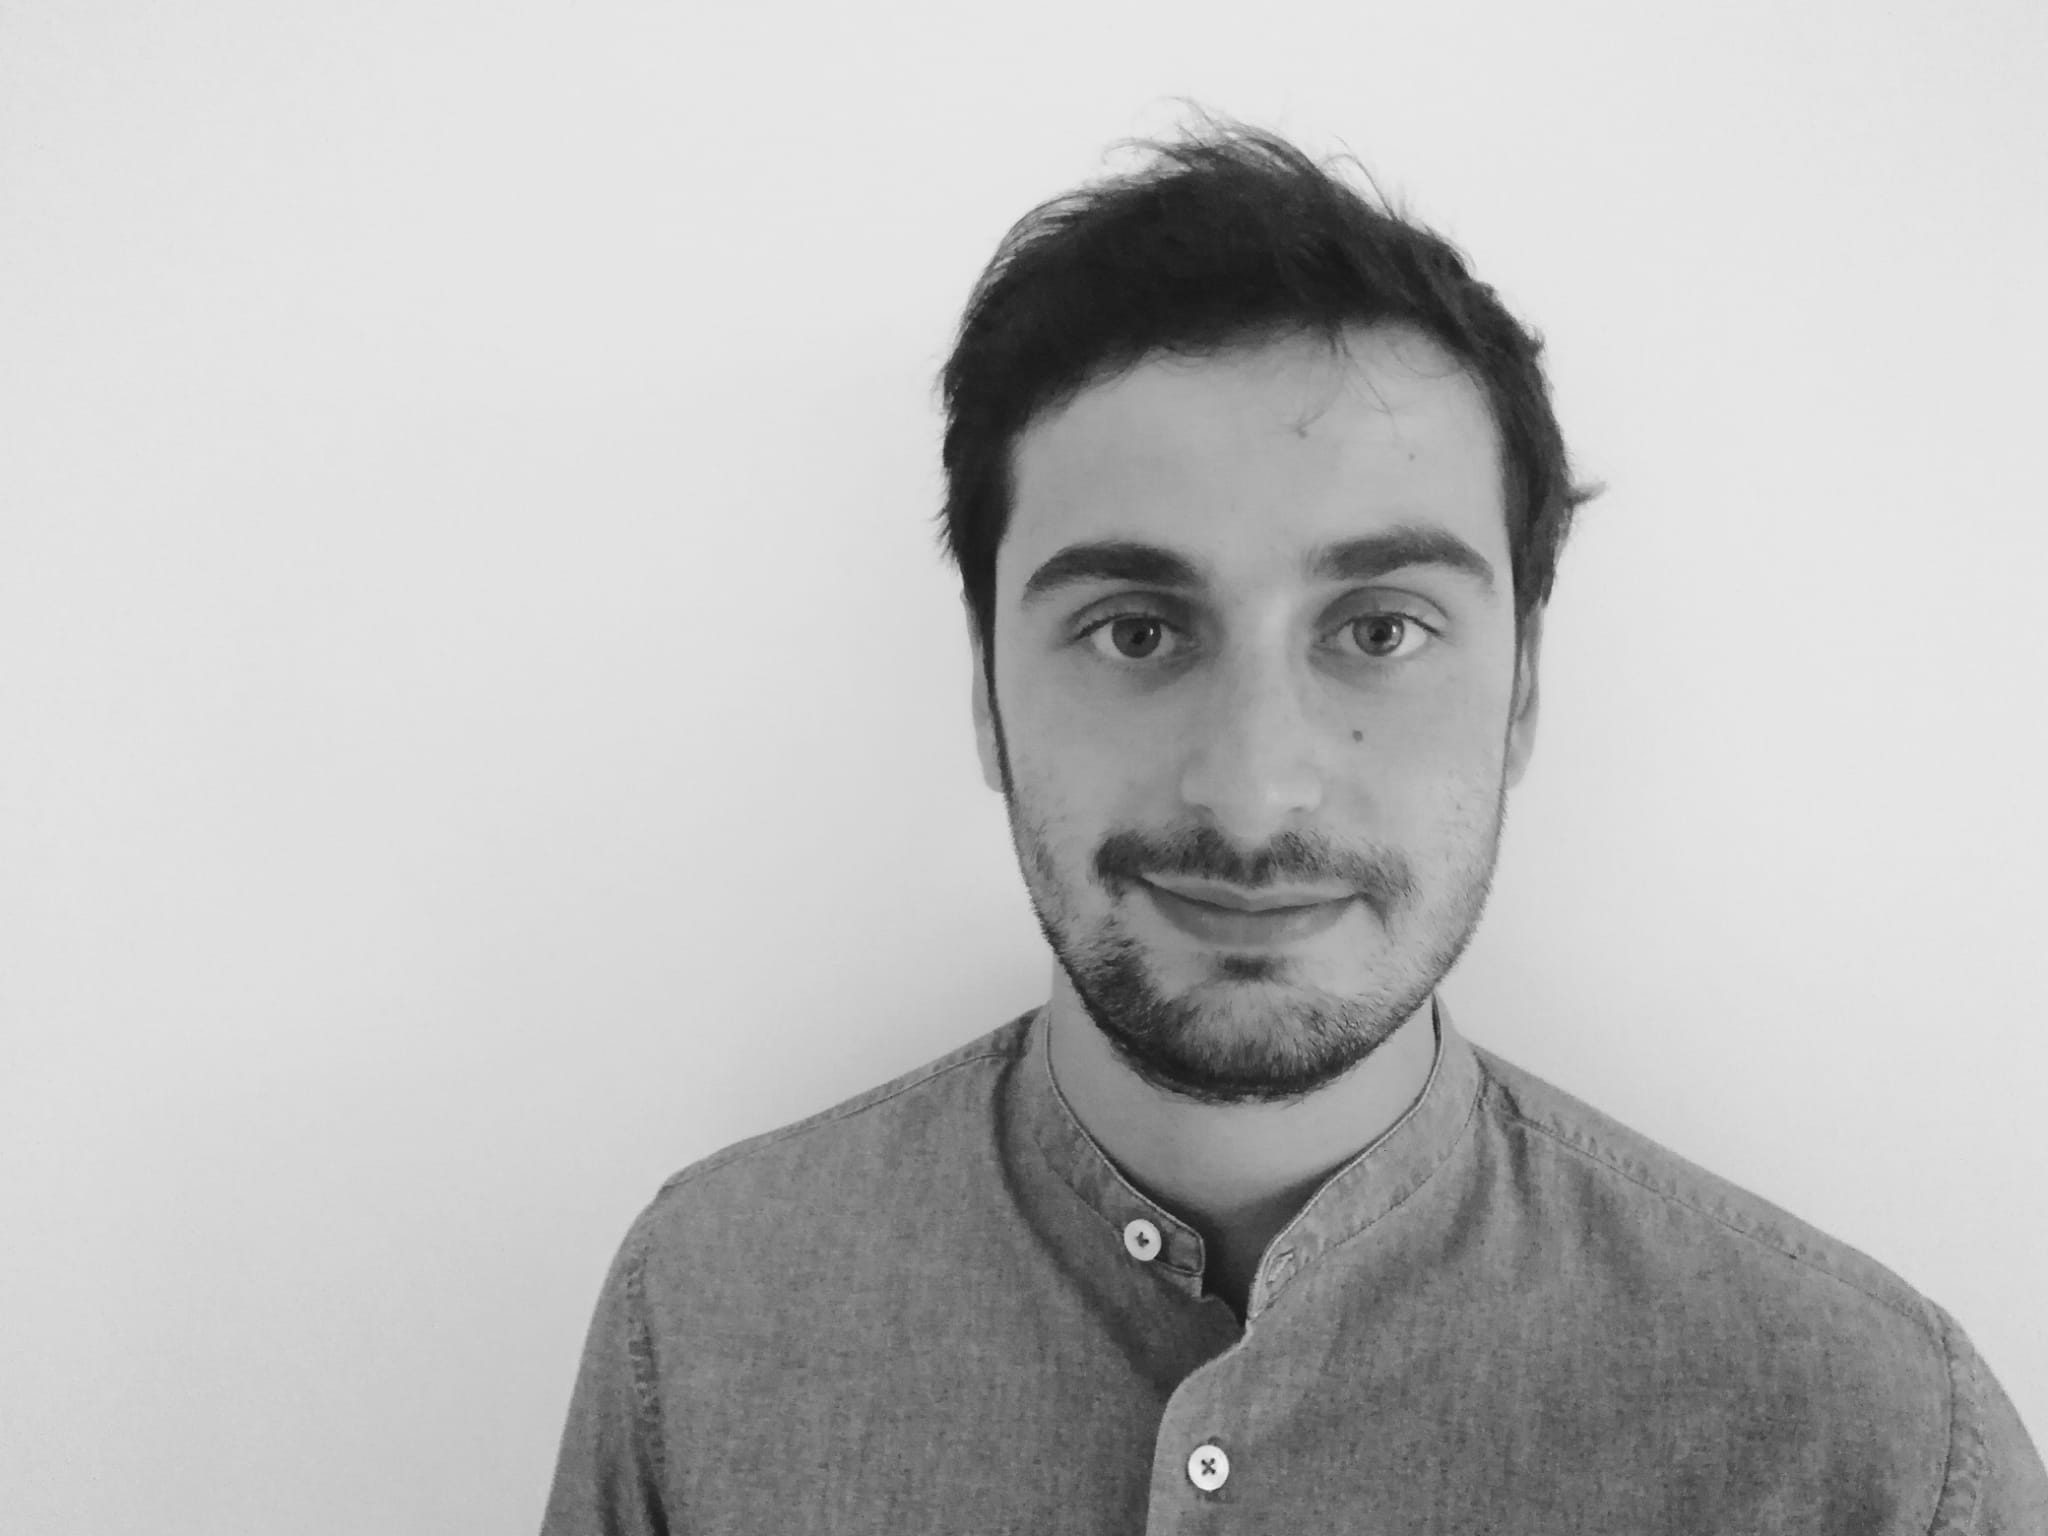
\includegraphics[scale=0.04]{cv_photo.jpeg}
\makecvtitle
\section{Education}
\cventry{2017--2020}{Master of Science in Physics (LM-17)}{Università degli Studi di Milano}{Italy}{}
{Relevant topics: Electroweak Interaction, Strong Interaction, Standard Model and Higgs sector, Quantum Field Theory and Renormalization, Particle Detectors. \\
Thesis title: "Measurement of differential cross sections for Higgs boson production in the $\gamma\gamma$ decay channel at $\sqrt{s} = 13$ TeV with the ATLAS experiment". \\
Supervisors: Prof. Marcello Fanti, Dott. Ruggero Turra \\
110/ 110 \\
CERN Document Server link: \url{https://cds.cern.ch/record/2746556?ln=en} \\
INFN Document Server link: \url{http://www.infn.it/thesis/thesis_dettaglio.php?tid=529318}}
\cventry{2018--2019}{Erasmus\scriptsize{+} \normalsize{exchange program}}{Albert-Ludwigs-Universität Freiburg}{Germany}{}
{Relevant topics: Advanced Particle Physics, Particle Detectors, Advanced Quantum Field Theory. \\
Period of stay:  October 2018 - March 2019}
\cventry{2012--2017}{Bachelor of Science in Physics (L-30)}{Università degli Studi di Milano}{Italy}{}
{Relevant topics: Classical Physics, Quantum Physics, Electromagnetism, Linear Algebra, Mathematical Analysis. \\ 
Thesis title: "Interferometria quantistica con elettroni e positroni: studio preliminare per esperimento QUPLAS". \\
Supervisors: Prof. Fabrizio Castelli, Prof. Marco Giammarchi, Dott. Simone Sala \\
94/ 110}
\cventry{2006--2011}{Diploma}{Liceo Classico G.D. Romagnosi}{Parma (PR)}{Italy}
{Maturità classica}

\section{Present research activities}
\cventry{2018--present}{Associate Member of the ATLAS Collaboration at CERN}{Geneva}{Switzerland}{}
{Currently I am working in the $H \rightarrow \gamma\gamma$ cross-sections working group within the ATLAS Collaboration. My contribution to the project consists in the development of a statistical analysis that explores and interprets the data collected by the ATLAS detector. This analysis has been implemented from scratch using the Python language and it is still mantained and released as a GIT repository. The code so far implemented is used as part of the official code machinery. This work is part of an analysis aimed at publishing an article by the ATLAS Collaboration}{}

\section{Past research activities}
\cventry{2020}{Measurement of differential cross sections for Higgs boson production in the $\gamma\gamma$ decay channel at $\sqrt{s} = 13$ TeV with the ATLAS experiment \small{(Master's degree)}}{}{}
{\newline CERN Document Server link: \url{https://cds.cern.ch/record/2746556?ln=en}}{}
\cventry{2017}{Quantum interferometry with electron and positron: a preliminary analysis for the QUPLAS experiment \small{(Bachelor's degree)}}{}{}{}{}

\section{Certifications}
\cventry{2020}{Data Analysis with Python}{Powered by IBM}{}{}{}
\cventry{2020}{Python for Data Science}{Powered by IBM}{}{}{}

\section{Language skills}
\cvitemwithcomment{Italian}{Mother tongue}{}
\cvitemwithcomment{English}{B2}{}
\cvitemwithcomment{German}{A2}{}

\section{Programming skills}
\cvitem{Languages \small{(advanced)}}{Python, Python3, \LaTeX}
\cvitem{Languages \small{(intermediate)}}{C++, Bash, XML, SQL}
\cvitem{Languages \small{(basic)}}{Mathematica, JavaScript, HTML4/5, CSS}
\cvitem{Tools \& frameworks}{ROOT, RDataFrame, PyROOT, RooFit, Jupyter Notebook, HTCondor, Python VirtualEnv, Numpy, Pandas, Matplotlib, Docker, MySQL, Git}

\vspace{4cm}
In compliance with the GDPR and the Italian Legislative Decree no. 196 dated 30/06/2003, I hereby authorize you to use and process my personal details contained in this document.
\end{document}
